% Copyright (C) Data Structures and Algorithms Team.
\documentclass[10pt,oneside,a4paper]{report}
\usepackage{url}
\usepackage{ifsym}
\begin{document}

\title{Data Structures and Algorithms\\Pseudocode}
\author{Granville Barnett\\Luca Del Tongo}
\maketitle

\newpage
\tableofcontents
\newpage

\section*{Preface}
This book consists of annotated pseudocode that was used when designing the algorithms which are contained in DSA\footnote{\url{http://codeplex.com/dsa}}. In DSA all implementations are in C\# \footnote{\url{http://msdn.microsoft.com/en-us/vcsharp/default.aspx}}.

The designs provided here serve as a reference for those who want to port well designed and tested implementations of common (and uncommon) data structures and algorithms to their imperative language of choice.

\pagestyle{headings}

\part{Data Structures}
% Copyright (C) Data Structures and Algorithms Team.
\chapter{Linked Lists}
Linked lists can be thought of from a high level perspective as being a series of nodes, each node has at least a pointer to the next node, and in the last nodes case a null pointer representing that there are no more nodes to follow.
The general characteristics of linked lists are as follows:

\begin{enumerate}
\item Insertion is $O(1)$
\item Deletion is $O(n)$
\item Searching is $O(n)$
\end{enumerate}

Out of the three operations the one that stands out is that of insertion, in DSA we chose to always maintain pointers (or more aptly references) to the node(s) at the head and tail of the linked list and so performing a traditional insertion to either the front or back of the linked list is an $O(1)$ operation. An exception to this rule is when performing an insertion before a node that is neither the head nor tail in a singly linked list, that is the node we are inserting before is somewhere in the middle of the linked list. It is apparent that in order to add before the designated node we need to traverse the linked list to acquire a pointer to the node before the node we want to insert before which yields an $O(n)$ runtime.

These data structure's are trivial, but they have a few key points which at times make them very attractive: 
\begin{inparaenum}
\item the list is dynamically resized, thus it incurs no copy penalty like an array or vector would eventually incur; and
\item insertion is $O(1)$.
\end{inparaenum}

\section{Singly Linked List}
Singly linked list's are one of the most primitive data structures you will find in this book, each node that makes up a singly linked list consists of a value, and a reference to the next node (if any) in the list. 

\subsection{Insertion}
In general when people talk about insertion with respect to linked lists of any form they implicitly refer to the adding of a node to the tail of the list, thus when you use an API like that of DSA and you see a general purpose method that adds a node to the list assume that you are adding that node to the tail of the list not the head.

Adding a node to a singly linked list has only two cases: 
\begin{inparaenum}
\item $head = \emptyset$ in which case the node we are adding is now both the $head$ and $tail$ of the list; or
\item we simply need to append our node onto the end of the list updating the $tail$ reference appropriately.
\end{inparaenum}

\begin{tabbing}
1)  \textbf{alg}\= \textbf{orithm} Add($value$) \\
2)  \> \textbf{Pre:}~~$value$ has passed custom type checks for type $T$ \\
3)  \> \textbf{Post:}~$value$ has been placed at the tail of the list \\
4)  \> $n \leftarrow$ node($value$) \\
5)  \> \textbf{if}~\= $head = \emptyset$ \\
6)  \> \> $head \leftarrow n$ \\
7)  \> \> $tail \leftarrow n$ \\
8)  \> \textbf{else} \\
9)  \> \> $tail$.Next $\leftarrow n$ \\
10) \> \> $tail \leftarrow n$ \\
11) \> \textbf{end if} \\
12) \textbf{end} Add \\
\end{tabbing}

\subsection{Searching}
Searching a linked list is straight forward, we simply traverse the list checking the value we are looking for with the value of each node in the linked list. The algorithm listed in this section is very similar to that used for traversal in \S\ref{singly_linked_traversal}.

\begin{tabbing}
1)  \textbf{alg}\= \textbf{orithm} Contains($head$, $value$) \\
2)  \> \textbf{Pre:}~~$head$ is the head node in the list \\
3)  \> ~~~~~~~~$value$ is the value to search for \\
4)  \> \textbf{Post:}~the item is either in the linked list, true; otherwise false \\
5)  \> $n \leftarrow head$ \\
6)  \> \textbf{whi}\= \textbf{le} $n~!= \emptyset$ \textbf{and} $n$.Value $!= value$ \\
7)  \> \> $n \leftarrow n$.Next \\
8)  \> \textbf{end while} \\
9)  \> \textbf{if} $n = \emptyset$ \\
10) \> \> \textbf{return false} \\
11) \> \textbf{else} \\
12) \> \> \textbf{return true} \\
13) \> \textbf{end if} \\
14) \textbf{end} Contains \\
\end{tabbing}

\subsection{Traversing the list} \label{singly_linked_traversal}
Traversing a singly list is the same as that of traversing a doubly linked list, you start at the head of the list and continue until you come across a node that is $\emptyset$. The two cases are as follows:
\begin{inparaenum}
\item $node = \emptyset$, we have exhausted all nodes in the linked list; or
\item we must update the $node$ reference to be $node$.Next.
\end{inparaenum}

The algorithm described is a very simple one that makes use of a simple $while$ loop to check the first case.

\begin{tabbing}
1)  \textbf{alg}\= \textbf{orithm} Traverse($head$) \\
2)  \> \textbf{Pre:}~~$head$ is the head node in the list \\
3)  \> \textbf{Post:}~the items in the list have been traversed \\
4)  \> $n \leftarrow head$ \\
5)  \> \textbf{whi}\=\textbf{le} $n~!= 0$ \\
6)  \> \> \textbf{yield} $n$.Value \\
7)  \> \> $n \leftarrow n$.Next \\
8)  \> \textbf{end while} \\
9)  \textbf{end} Traverse \\
\end{tabbing}

\section{Doubly Linked List}

% Copyright (C) Data Structures and Algorithms Team.
\chapter{Binary Search Tree}

% Copyright (C) Data Structures and Algorithms Team.
\chapter{Heap}

% Copyright (C) Data Structures and Algorithms Team.
\chapter{Sets}
\section{Unordered}
\section{Ordered}

% Copyright (C) Data Structures and Algorithms Team.
\chapter{Queues}
Queues are an essential data structure that have found themselves used in vast amounts of software from user mode to kernel mode applications that are core to the system. Fundamentally they honour a first in first out (FIFO) strategy, that is the item first put into the queue will be the first served, the second item added to the queue will be the second to be served and so on.

All queues only allow you to access the item at the front of the queue, when you add an item to the queue that item is placed at the back of the queue.

Historically queues always have the following three core methods:

\begin{description}
\item[Enqueue:] places an item at the back of the queue;
\item[Dequeue:] retrieves the item at the front of the queue, and removes it from the queue;
\item[Front:] retrieves the item at the front of the queue without removing it from the queue
\end{description}

As an example to demonstrate the behaviour of a queue we will walk through a scenario whereby we invoke each of the previously mentioned methods observing the mutations upon the queue data structure, the following list describes the operations performed upon the queue in Figure \ref{fig:queue_mutations}:

\begin{enumerate}
\item Enqueue($10$)
\item Enqueue($12$)
\item Enqueue($9$)
\item Enqueue($8$)
\item Enqueue($3$)
\item Dequeue()
\item Front()
\item Enqueue($33$)
\item Front()
\item Dequeue()
\end{enumerate}

\begin{figure}
\begin{center}
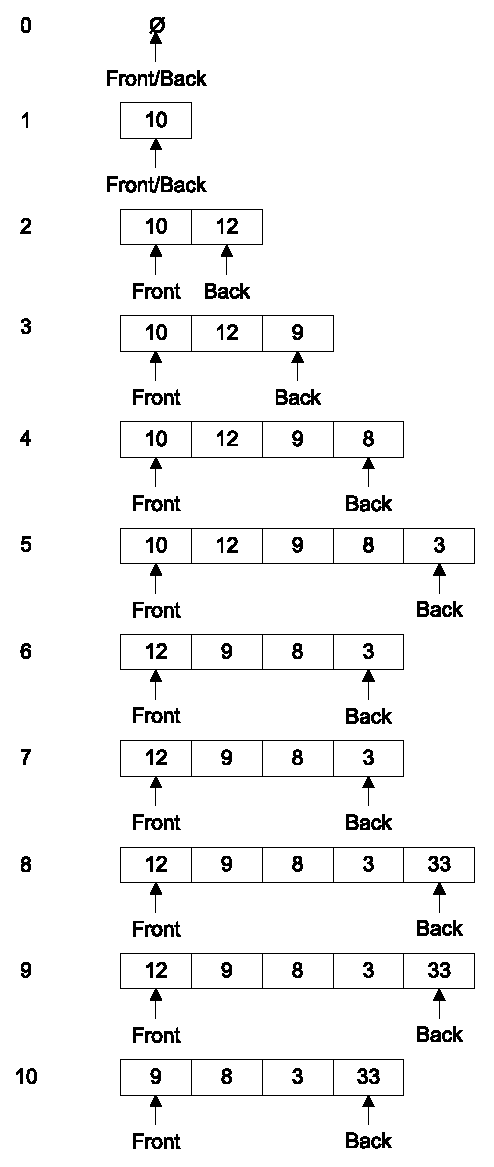
\includegraphics{queue_mutations}
\end{center}
\caption{Queue mutations} \label{fig:queue_mutations}
\end{figure}

\section{Standard Queue}
A queue is implicitly like that described prior to this section, in DSA we don't provide a standard queue because queues are so popular and such a core data structure you will find that pretty much every mainstream library provides a queue data structure that you can use with your language of choice. In this section we will discuss how you can, if required implement an efficient queue data structure.

The main property of a queue is that we have access to the item at the front of the queue, the queue data structure can be efficiently implemented using a singly linked list (defined in \S\ref{singly_linked_list}). A singly linked list provides $O(1)$ insertion, and deletion run time complexities - the reason we have an $O(1)$ run time complexity for deletion is because we only ever in a queue remove the item at the front (Dequeue) and since we always have a pointer to the item at the head of a singly linked list removal is simply a case of returning the value of the old head node, and then modifying the head pointer to be the next node of the old head node. The run time complexity for searching a queue remains the same as that of a singly linked list, $O(n)$.

\section{Priority Queue}
Unlike a standard queue where items are ordered in terms of who arrived first, a priority queue determines the order of its items by using a form of custom comparer to see which item has the highest priority. Other than the items in a priority queue being ordered by priority it remains the same as a normal queue, you can only access the item at the front of the queue.

A sensible implementation of a priority queue is to use a heap data structure (defined in \S\ref{heap}). Using a heap we can look at the first item in the queue by simply returning the item at index $0$ within the heap array. A heap provides us with the ability to construct a priority queue where by the items with the highest priority are either those with the smallest value, or those with the largest.

% Copyright (C) Data Structures and Algorithms Team.
\chapter{Balanced Trees} 
\section{AVL Tree} \label{Avl}


\part{Algorithms}
% Copyright (C) Data Structures and Algorithms Team.
\chapter{Sorting}
All the sorting algorithms in this chapter use data structures of a specific type to demonstrate sorting, e.g. a $32$ bit integer is often used as its associated operations (e.g. $<$, $>$, etc) are clear in their behaviour.

The algorithms discussed can easily be translated into generic sorting algorithms within your respective language of choice.
\newpage
\section{Bubble Sort}
One of the most simple forms of sorting is that of comparing each item with every other item in some list, however as the description may imply this form of sorting is not particularly effecient $O(n^{2})$. In it's most simple form bubble sort can be implemented as two loops.

\begin{figure}[h]
\begin{center}
\includegraphics{sorting_bubble}
\end{center}
\caption{Bubble Sort Iterations} \label{fig:sorting_bubble}
\end{figure}

\begin{tabbing}
1)  \textbf{alg}\= \textbf{orithm} BubbleSort($list$) \\
2)  \> \textbf{Pre:}~~$list~!= \emptyset$ \\
3)  \> \textbf{Post:}~$list$ has been sorted into values of ascending order \\
4)  \> \textbf{for}\=~$i \leftarrow 0$ to $list.Count - 1$ \\
5)  \> \> \textbf{for}\=~$j \leftarrow 0$ to $list.Count - 1$ \\
6)  \> \> \> \textbf{if}~\= $list[i] < list[j]$ \\
7)  \> \> \> \> $Swap(list[i], list[j])$ \\
8)  \> \> \> \textbf{end if} \\
9)  \> \> \textbf{end for} \\
10) \> \textbf{end for} \\
11) \> \textbf{return} $list$ \\
12) \textbf{end} BubbleSort
\end{tabbing}

\newpage
\section{Merge Sort}
Merge sort is an algorithm that has a fairly effecient space time complexity - $O(n~log~n)$ and is fairly trivial to implement. The algorithm is based on splitting a list, into two similar sized lists ($left$, and $right$) and sorting each list and then merging the sorted lists back together. \textit{Note: the function MergeOrdered simply takes two ordered lists and makes them one.}

\begin{figure}[h]
\begin{center}
\includegraphics{sorting_merge}
\end{center}
\caption{Merge Sort Divide et Impera Approach} \label{fig:sorting_merge}
\end{figure}

\begin{tabbing}
1)  \textbf{alg}\= \textbf{orithm} Mergesort($list$) \\
2)  \> \textbf{Pre:}~~$list~!=~\emptyset$ \\
3)  \> \textbf{Post:}~$list$ has been sorted into values of ascending order \\
4)  \> \textbf{if}~\= $list$.Count $= 1$ // already sorted \\
5)  \> \> \textbf{return}~$list$ \\
6)  \> \textbf{end if} \\
7)  \> $m \leftarrow list$.Count $/~2$ \\
8)  \> $left \leftarrow$ list($m$) \\
9)  \> $right \leftarrow$ list($list$.Count $-~m$) \\
10) \> \textbf{for}\=~$i \leftarrow 0$ to $left$.Count$-1$ \\
11) \> \> $left$[$i$] $\leftarrow$ list[$i$] \\
12) \> \textbf{end for} \\
13) \> \textbf{for}\=~$i \leftarrow 0$ to $right$.Count$-1$ \\
14) \> \> $right$[$i$] $\leftarrow$ list[$i$] \\
15) \> \textbf{end for} \\
16) \> $left \leftarrow$ Mergesort($left$) \\
17) \> $right \leftarrow$ Mergesort($right$) \\
18) \> \textbf{return} MergeOrdered($left$, $right$) \\
19) \textbf{end} Mergesort \\
\end{tabbing}

\newpage
\section{Quick Sort} 
Quick sort is one of the most popular sorting algorithms based on divide et impera strategy, resulting in an $O(n~log~n)$ complexity. The algorithm starts by picking an item, called pivot, and moving all smaller items before it, while all greater elements after it. This is the main quick sort operation, called partition, recursively repeated on lesser and greater sub lists until their size  is one or zero - in which case the list is implicitly sorted.

Choosing an appropriate pivot, as for example the median element is fundamental for avoiding the drastically reduced performance of $O(n^{2})$.

\begin{tabbing}
1)  \textbf{alg}\= \textbf{orithm} QuickSort($list$) \\
2)  \> \textbf{Pre:}~~$list~!=~\emptyset$ \\
3)  \> \textbf{Post:}~$list$ has been sorted into values of ascending order \\
4)  \> \textbf{if}~\= $list$.Count $= 1$ // already sorted \\
5)  \> \> \textbf{return}~$list$ \\
6)  \> \textbf{end if} \\
7)  \> $pivot \leftarrow $MedianValue($list$) \\
8)  \> \textbf{for}\=~$i \leftarrow 0$ to $list$.Count$-1$ \\
9)  \> \> \textbf{if}~\= $list[i] = pivot$ \\
10) \> \> \> $equal$.Insert$(list[i])$\\
11) \> \> \textbf{end if} \\
12) \> \> \textbf{if}~\= $list[i] < pivot$ \\
13) \> \> \> $less$.Insert$(list[i])$\\
14) \> \> \textbf{end if} \\
15) \> \> \textbf{if}~\= $list[i] > pivot$ \\
16) \> \> \> $greater$.Insert$(list[i])$\\
17) \> \> \textbf{end if} \\
18) \> \textbf{end for} \\
19) \> \textbf{return} Concatenate(QuickSort($less$),~$equal$,~QuickSort($greater$)) \\
20) \textbf{end} Quicksort \\
\end{tabbing}

\newpage
\section{Insertion Sort} \label{shell_sort}
Insertion sort is a somewhat interesting algorithm with an expensive runtime of $O(n^{2})$. It can be best thought of as a sorting scheme similar to that of sorting a hand of playing cards, i.e. you take one card and then look at the rest with the intent of building up an ordered set of cards in your hand.

\begin{tabbing}
1)  \textbf{alg}\= \textbf{orithm} Insertionsort($list$) \\
2)  \> \textbf{Pre:}~~ $list~!=~\emptyset$ \\
3)  \> \textbf{Post:}~$list$ has been sorted into values of ascending order \\
4)  \> $unsorted \leftarrow 1$ \\
5)  \> \textbf{whi}\= \textbf{le} $unsorted < list$.Count \\
6)  \> \> $hold \leftarrow list$[$unsorted$] \\
7)  \> \> $i \leftarrow unsorted - 1$ \\
8)  \> \> \textbf{whi}\= \textbf{le} $i \geq 0$ \textbf{and} $hold < list$[$i$] \\
9)  \> \> \> $list$[$i + 1$] $\leftarrow$ $list$[$i$] \\
10) \> \> \> $i \leftarrow i - 1$ \\
11) \> \> \textbf{end while} \\
12) \> \> $list$[$i+1$] $\leftarrow hold$ \\
13) \> \> $unsorted \leftarrow unsorted + 1$ \\
14) \> \textbf{end while} \\
15) \> \textbf{return} $list$ \\
16) \textbf{end} Insertionsort \\
\end{tabbing}

\newpage
\section{Shell Sort}
Put simply shell sort can be thought of as a more efficient variation of insertion sort as described in \S\ref{shell_sort}, it achieves this mainly by comparing items of varying distances apart resulting in a run time complexity of $O(n~log^{2}~n)$.

Shell sort is fairly straight forward but may seem somewhat confusing at first as it differs from other sorting algorithms in the way it selects items to compare. 

\begin{tabbing}
1)  \textbf{alg}\= \textbf{orithm} ShellSort($list$) \\
2)  \> \textbf{Pre:}~~$list~!=~\emptyset$ \\
3)  \> \textbf{Post:}~$list$ has been sorted into values of ascending order \\
4)  \> $increment \leftarrow list$.Count $/~2$ \\
5)  \> \textbf{whi}\= \textbf{le} $increment~!= 0$ \\
6)  \> \> $current \leftarrow increment$ \\
7)  \> \> \textbf{whi}\= \textbf{le} $current < list$.Count \\
8)  \> \> \> $hold \leftarrow list$[$current$] \\
9)  \> \> \> $i \leftarrow current - increment$ \\
10) \> \> \> \textbf{whi}\= \textbf{le} $i \geq 0$ \textbf{and} $hold < list$[$i$] \\
11) \> \> \> \> $list$[$i + increment$] $\leftarrow list$[$i$] \\
12) \> \> \> \> $i -= increment$ \\
13) \> \> \> \textbf{end while} \\
14) \> \> \> $list$[$i + increment$] $\leftarrow hold$ \\
15) \> \> \> $current \leftarrow current + 1$ \\
16) \> \> \textbf{end while} \\
17) \> \> $increment~/= 2$ \\
18) \> \textbf{end while} \\
19) \> \textbf{return} $list$ \\
20) \textbf{end} ShellSort \\
\end{tabbing}


% Copyright (C) Data Structures and Algorithms Team.
\chapter{Numeric}
Unless stated otherwise the alias $n$ denotes a standard $32$ bit integer.

\section{Primality Test} \label{cha:Primality}
A simple algorithm that determines whether or not a given integer is a prime number, e.g. $2$, $5$, $7$, and $13$ are \textbf{all} prime numbers, however $6$ is not as it can be the result of the product of two numbers that are $< 6$.

In an attempt to slow down the inner loop the $\sqrt{n}$ is used as the upper bound.

\begin{tabbing}
1) \textbf{alg}\= \textbf{orithm} IsPrime($n$)\\
2) \> \textbf{Post:} $n$ is determined to be a prime or not \\
3) \> \textbf{for} \= $i \leftarrow 2$ \textbf{to} $n$ \textbf{do}\\
4) \> \> \textbf{for} \= $j \leftarrow 1$ \textbf{to} $sqrt(n)$ \textbf{do}\\
5) \> \> \> \textbf{if}~\= $i * j = n$\\
6) \> \> \> \> \textbf{return} false\\
7) \> \> \> \textbf{end if}\\
8) \> \> \textbf{end for}\\	
9) \> \textbf{end for}\\
10) \textbf{end} IsPrime
\end{tabbing}

\section{Base conversions}
DSA contains a number of algorithms that convert a base $10$ number to its equivalent binary, octal or hexadecimal form. For example $78_{10}$ has a binary representation of $1001110_{2}$.

\begin{tabbing}
1) \textbf{alg}\= \textbf{orithm} ToBinary($n$)\\
2) \> \textbf{Pre:}~~$n \geq 0$ \\
3) \> \textbf{Post:}~$n$ has been converted into its base $2$ representation \\
4) \> \textbf{whi}\= \textbf{le} $n > 0$\\
5) \> \> $list.Add(n~\%~2)$\\
6) \> \> $n \leftarrow n / 2$\\
7) \> \textbf{end while}\\
8) \textbf{end} ToBinary\\
\end{tabbing}

% Copyright (C) Data Structures and Algorithms Team.
\chapter{Searching}

\section{Sequential Search}
A simple algorithm that search for a specific item inside a list. It operates looping on each element $O(n)$ until a match occurs or the end is reached.

\begin{tabbing}
1) \textbf{alg}\= \textbf{orithm} SequentialSearch($list$, $item$)\\
2) \> \textbf{Pre:}~~ $list~!=~\emptyset$ \\
3) \> \textbf{Post:}~ return $index$ of item if found, otherwise $-1$ \\
4) \> \= $index \leftarrow 0$ \\
5) \> \textbf{whi}\= \textbf{le} $index < list$.Count  \textbf{and} $list$[$index$]~!= $item$ \\
6) \> \> \= $index \leftarrow index+1$ \\
7) \> \textbf{end while} \\
8) \> \textbf{if }\= $ index < list$.Count  \textbf{and} $list$[$index$] = $item$ \\
9) \> \> \textbf{return} $index$ \\
10)\> \textbf{end if} \\
11)\> \textbf{return} $-1$ \\ 
12) \textbf{end} SequentialSearch \\

\end{tabbing}

\section{Probability Search}
Probability Search is a statistical sequential search algorithm. In addition to search for an \textbf{item}, it takes into account its \textbf{frequency} by swapping it with it's predecessor in the list. The algorithm complexity still remain an $O(n)$ but in a non-uniform items search the more frequent items are in the first positions, reducing list scanning time.

\begin{tabbing}
1) \textbf{alg}\= \textbf{orithm} ProbabilitySearch($list$, $item$)\\
2) \> \textbf{Pre:}~~ $list~!=~\emptyset$ \\
3) \> \textbf{Post:}~ a boolean indicating where the item is found or not;\\
   \>~~~~~~~~~ in the former case swap founded item with its predecessor \\
4) \> \= $index \leftarrow 0$ \\
5) \> \textbf{whi}\= \textbf{le} $index < list$.Count  \textbf{and} $list$[$index$]~!= $item$ \\
6) \> \> \= $index \leftarrow index+1$ \\
7) \> \textbf{end while} \\
8) \> \textbf{if }\= $ index \geq list$.Count  \textbf{or} $list$[$index$] ~!= $item$ \\
9) \> \> \textbf{return} false \\
10)\> \textbf{end if} \\
11)\> \textbf{if }\= $ index > 0$ \\
12)\> \> $Swap(list[index], list[index-1])$ \\
13)\> \textbf{end if } \\
14)\> \textbf{return} true \\ 
15) \textbf{end} ProbabilitySearch \\
\end {tabbing}

% Copyright (C) Data Structures and Algorithms Team.
\chapter{Sets}

% Copyright (C) Data Structures and Algorithms Team.
\chapter{Strings}
Strings have their own chapter in this text purely because string operations and transformations are incredibly frequent within programs. The algorithms presented are based on problems the authors have come across previously, or were formulated to satisfy curiosity.

\section{Reversing the order of words in a sentence}
Defining algorithms for primitive string operations is simple, e.g. extracting a substring of a string, however some algorithms that require more inventiveness can be a little more tricky.

The algorithm presented here does not simply reverse the characters in a string, rather it reverses the order of words within a string. This algorithm works on the principal that words are all delimited by whitespace, and using a few markers to define where words start and end we can easily reverse them.

\begin{tabbing}
1) \textbf{alg}\= \textbf{orithm} ReverseWords($value$) \\
2) \> \textbf{Pre:}~~ $value~!= \emptyset$, $sb$ is a string buffer \\
3) \> \textbf{Post:}~ the words in $value$ have been reversed \\
4) \> $last \leftarrow value$.Length $-~1$ \\
5) \> $start \leftarrow last$ \\
6) \> \textbf{whi}\= \textbf{le} $last \geq 0$ \\
7) \> \> // skip whitespace \\
8) \> \> \textbf{whi}\= \textbf{le} $start \geq 0$ \textbf{and} $value$[$start$] = whitespace \\
9) \> \> \> $start \leftarrow start - 1$ \\
10)\> \> \textbf{end while} \\
11)\> \> $last \leftarrow start$ \\
12)\> \> // march down to the index before the beginning of the word \\
13)\> \> \textbf{while} $start \geq 0$ \textbf{and} $start~!=$ whitespace \\
14)\> \> \> $start \leftarrow start - 1$ \\
15)\> \> \textbf{end while} \\
16)\> \> // append chars from $start + 1$ to $length + 1$ to string buffer sb \\
17)\> \> \textbf{for} $i \leftarrow start + 1$ \textbf{to} $last$ \\
18)\> \> \> $sb$.Append($value$[$i$]) \\
19)\> \> \textbf{end for} \\
20)\> \> // if this isn't the last word in the string add some whitespace after the word in the buffer \\
21)\> \> \textbf{if} $start > 0$ \\ 
22)\> \> \> $sb$.Append(` ') \\
23)\> \> \textbf{end if} \\
24)\> \> $last \leftarrow start - 1$ \\
25)\> \> $start \leftarrow last$ \\
26)\> \textbf{end while} \\
27)\> // check if we have added one too many whitespace to $sb$ \\
28)\> \textbf{if} $sb$[$sb$.Length $- 1$] = whitespace \\
29)\> \> // cut the whitespace \\
30)\> \> $sb$.Length $\leftarrow sb$.Length $- 1$ \\
31)\> \textbf{end if} \\
32)\> \textbf{return} $sb$ \\
33) \textbf{end} ReverseWords \\
\end{tabbing}


\appendix
% Copyright (C) Data Structures and Algorithms Team.
\chapter{Translation Walkthrough}
The conversion from pseudo to an actual imperative language is usually very straight forward, to clarify an example is provided.
In this example we will convert the algorithm in \S\ref{cha:Primality} to the C\# language.

\begin{tabbing}
1) pub\=lic static bool IsPrime(int number) \\
2) \{ \\
3) \> if (\=number $<$ 2) \\
4) \> \{ \\
5) \> \> return false; \\
6) \> \{ \\ 
7) \> int innerLoopBound $=$ (int)Math.Floor(Math.Sqrt(number)); \\
8) \> for (int i $=$ 1; i $<$ number; i++) \\
9) \> \{ \\
10) \> \> for\= (int j $=$ 1; j $<=$ innerLoopBound; j++) \\
11) \> \> \{ \\
12) \> \> \> if (\=i $*$ j $==$ number) \\
13) \> \> \> \{ \\
14) \> \> \> \> return false; \\
15) \> \> \> \} \\
16) \> \> \} \\
17) \> \} \\
18) \> return true; \\
19) \} \\
\end{tabbing}

For the most part the conversion is a straight forward process, however you may have to inject various calls to other utility algorithms to ascertain the correct result.

A consideration to take note of is that many algorithms have fairly strict preconditions, of which there may be several - in these scenarios you will need to inject the correct code to handle such situations to preserve the correctness of the algorithm. Most of the preconditions can be suitably handled by throwing the correct exception.

% Copyright (C) Data Structures and Algorithms Team.
\chapter{Symbol Definitions}
Throughout the pseudocode listings you will find several symbols used,  describes the meaning of each of those symbols.

\begin{table}[h]
\begin{center}
\begin{tabular}[t]{|c|l|}
\hline
\textbf{Symbol} & \textbf{Description} \\
\hline
$\leftarrow$ & Assignment. \\
\hline
$=$ & Equality. \\
\hline
$\leq$ & Less than or equal to.  \\
\hline
$<$ & Less than.* \\
\hline
$\geq$ & Greater than or equal to.  \\
\hline
$>$ & Greater than.* \\
\hline
$!=$ & Inequality. * \\
\hline
$\emptyset$ & Null. \\
\hline
\textbf{and} & Logical and.  \\
\hline
\textbf{or} & Logical or.  \\ 
\hline
whitespace & Single occurrence of whitespace. \\
\hline
\textbf{yield} & Like \textbf{return} but builds a sequence. \\
\hline
\end{tabular}
\end{center}
\caption{Pseudo symbol definitions}
\end{table}

* This symbol has a direct translation with the vast majority of imperative counterparts.


\end{document}
